\chapter{Introduzione}\label{ch:intro}

\section{Descrizione del problema}
Il problema analizzato consiste nel fornire in tempo reale a un agente un'approssimazione del cammino migliore per i suoi clienti.
La topologia dei clienti viene fornita dall'utente in modo tale da poterla aggiornare in base alle sue necessit\`a.
A tal fine viene proposta una soluzione basata sull'algoritmo di ``Ant Colony Optimization'' (\textbf{ACO}).

\subsection{Funzionalità del sistema}
Illustriamo a seguire la nostra proposta:
\begin{itemize}
    \item l'utente può interfacciarsi al sistema per inserire i clienti e i costi per spostarsi tra quest'ultimi;
    \item il sistema crea un grafo e computa un'approssimazione del percorso migliore;
    \item tramite l'interfaccia grafica viene visualizzato il grafo e il percorso;
    \item l'utente può fornire nuovi dati sui clienti e/o i costi;
    \item il sistema si aggiorna mostrando il nuovo percorso all'agente.
\end{itemize}

Il sistema si presuppone di essere in continua esecuzione e che l'approssimazione del percorso migliore sia adeguata.

Infine, la soluzione proposta è applicabile anche ad altri contesti, con pochi adattamenti necessari, se non nessuno.
Uno di questi contesti potrebbe essere un sistema di veicoli autonomi, in cui quest'ultimi si muovono all'interno di un'area,
comunicandosi informazioni riguardanti lo stato dei percorsi e dove trovare i percorsi migliori.
\newpage
\section{Struttura dell'applicazione}
L'applicazione è composta dai seguenti elementi:
\begin{itemize}
    \item il sistema ACO distribuito è il modulo logico per computare l'approssimazione del TSP;
    \item un'interfaccia grafica per poter visualizzare il grafo e il cammino calcolato;
    \item un modulo intermedio tra sistema ACO, l'interfaccia grafica e le interazioni dell'utente (API);
    \item un agente (o multipli) che utilizza l'interfaccia grafica;
    \item un utente (o un sistema) che interagisce con il modulo intermedio, per aggiungere o rimuovere clienti e modificare informazioni sui percorsi.
\end{itemize}
Da questo punto in poi, con \textit{agente} si intenderà l'ente che usa l'interfaccia grafica, mentre con \textit{utente} si intende solamente chi utilizza le API del sistema.

\begin{figure}[t]
    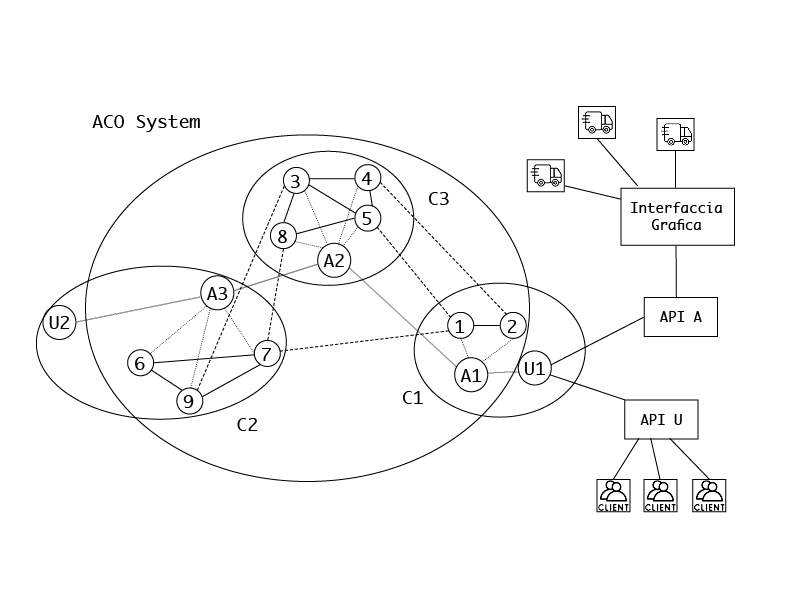
\includegraphics[width=\textwidth]{images/aco_system.png}    
    \centering
    \caption{Topologia del sistema: l'ACO system è composto da dei cluster identificati dalla lettera \texttt{C}, che contengono dei nodi agente identificati dalla lettera \texttt{A}. I nodi agenti dispongono di un piccolo sottoinsieme dei nodi del grafo rappresentati dai numeri. I nodi identificati con la lettera \texttt{U} sono i nodi utente.}
    \label{fig:acosystem}
\end{figure}

\subsection{Struttura distribuita}
Il sistema ACO è un sistema distribuito peer-to-peer, i cui nodi non necessariamente hanno una conoscenza completa della topologia. 
All'interno del sistema possono essere presenti più nodi su una stessa macchina (fisica o virtuale).

I nodi, idempotenti, possono essere di due tipi:
\begin{itemize}
    \item nodo utente: aggiorna il grafo dei clienti e riceve informazioni sul grafo;
    \item nodo ACO: gestisce i nodi del grafo dei clienti e partecipa alla computazione dell'algoritmo.
\end{itemize}

La comunicazione tra nodi è generalmente \textbf{asincrona}, ad eccezione di operazione da parte dell'utente, e \textbf{accoppiata} rispetto sia al \textbf{tempo} che allo \textbf{spazio}.
Questo perché un nodo invia un messaggio a un suo vicino (specifico), il quale deve esistere nello stesso momento, senza però dover attendere una risposta.

I clienti sono rappresentati come nodi di un grafo pesato non orientato, in cui il peso degli archi rappresenta il costo di spostarsi da un cliente all'altro.
Ogno nodo del sistema ACO gestisce un sottoinsieme dei clienti presenti.

La topologia del sistema è quindi un grafo non orientato composto da nodi ACO e nodi utente, come in figura \ref{fig:acosystem}.

\subsection{Algoritmi e CAP theorem}
Considerando il CAP theorem, si è scelto di assicurare disponibilità (\textbf{availability}) e tolleranza rispetto alle partizioni (\textbf{partition tolerance}).
Questo perché è necessario che il sistema sia sempre responsivo e possa funzionare anche se un nodo è soggetto a malfunzionamenti.
Nel caso di un'azienda di dimensioni ridotte potrebbe essere preferibile implementare un sistema consistente piuttosto che disponibile,
poiché il grafo dei clienti non riceverebbe frequenti aggiornamenti. Nel nostro caso, invece, supponiamo di lavorare per
un'azienda sufficientemente grande, con una discreta dinamicità dei clienti. Risulta quindi più importante poter aggiornare
il grafo velocemente rispetto al fatto che l'intero sistema abbia le informazioni più recenti.

Al fine di visualizzare il grafo ACO globale, tramite interfaccia grafica, è necessario che tutti i nodi pubblicizzino i propri
dati. È stato quindi pensato di utilizzare una variante dell'ECHO algorithm. 
Un nodo utente viene notificato da un nodo ACO quando finisce un round del percorso effettuato e propaga l'informazione tramite echo a tutti
gli altri nodi utente. 
L'algoritmo viene usato anche durante l'inizializzazione del sistema per informare tutti i nodi utente dei nodi
del grafo. Infine, esso viene utilizzato anche per l'aggiunta e rimozione di nodi del grafo.

Per aggiornare il grafo dei clienti, è stato scelto di utilizzare un sistema a \textit{ticket}.
L'utente, per poter effettuare un aggiornamento, deve chiedere un ticket.
Verrà quindi mandato un messaggio al nodo ACO a cui è collegato, che lo inoltrerà al \textit{ticket master}.
Il ticket master risponderà quindi inviando il ticket, che l'utente potrà usare per fare richiesta di aggiornare il grafo.
Questo sistema serve per assicurare che gli aggiornamenti vengano fatti in ordine, ad esempio se un utente decide di aggiungere un nodo,
non deve essere possibile che un altro utente possa rimuoverlo prima che questo aggiornamento sia noto a tutti i nodi ACO.

Il ticket master è un nodo ACO che viene eletto tramite un algoritmo echo con extinction.
Ogni nodo ACO inizia un echo, allegando il proprio ID e scarta tutti gli ``echi'' con ID minore al proprio.
Se invece riceve un echo con ID maggiore, terminerà il proprio e parteciperà a quello appena ricevuto.
Alla fine, tutti gli ``echi'' tranne quello con ID maggiore verrano terminati senza successo e l'iniziatore sarà il leader.

\section{Trasparenze del sistema}\label{sec:tra}
È stato scelto di implementare le seguenti trasparenze:
\begin{itemize}
    \item \textit{access transparency}: l'utente può aggiungere o rimuovere nodi del grafo senza sapere se questi si trovano in locale o in remoto;
    \item \textit{location transparency}: l'utente non ha conoscenza della posizione fisica e/o della posizione nella rete degli altri nodi;
    \item \textit{concurrency transparency}: i nodi operano sullo stesso grafo in contemporanea senza interferire tra loro;
    \item \textit{scaling transparency}: nuovi nodi possono essere aggiunti al sistema senza che questo subisca variazioni o interruzioni;
    \item \textit{failure transparency}: terminazioni inaspettate di nodi del sistema non portano a interruzioni del servizio per l'utente. 
\end{itemize}
Le rimanenti trasparenze non sono state implementate perché non inerenti alla richiesta.

\section{Piano di testing}
Il sistema verrà testato su diversi grafi casuali, statici e dinamici. Verrà inoltre testata la resilienza del sistema a cambiamenti della topologia
e interruzioni inaspettate dei nodi.

Altro oggetto di testing sarà l'osservazione di quanti round (per nodo), in media, sono necessari per raggiungere la convergenza al percorso migliore.

\section{Piano di sviluppo}
Lo sviluppo seguirà le seguenti fasi:
\begin{itemize}
    \item progettazione del sistema e dei casi d'uso;
    \item specificazione dei modelli di comunicazione del sistema;
    \item progettazione interfaccia grafica;
    \item progettazione dell'implementazione del sistema ACO e dell'interfaccia;
    \item scrittura casi di test;
    \item implementazione in Erlang del sistema ACO;
    \item testing sistema ACO;
    \item implementazione dell'interfaccia grafica;
    \item testing e validazione finale.
\end{itemize}